\documentclass[a4paper,12pt]{article}
\usepackage[utf8]{inputenc}
\usepackage[russian]{babel}
\usepackage{amsmath, amssymb}
\usepackage[hyperfootnotes=false]{hyperref}
\usepackage{geometry}
\usepackage{indentfirst}
\usepackage{graphicx}
\usepackage{float}
\usepackage{enumitem}
\usepackage{caption}
\usepackage{array}
\geometry{
	a4paper,
	top=24mm,
	bottom=30mm,
	left=20mm,
	right=20mm
}

\newcommand{\blfootnote}[1]{%
	\begingroup
	\renewcommand{\thefootnote}{}%
	\footnote{#1}%
	\addtocounter{footnote}{-1}%
	\endgroup
}

% Отступ первой строки абзаца 1 см
\setlength{\parindent}{1cm}
\setlength{\parskip}{0pt}
\linespread{1}                 % одинарный интервал

% Отключение нумерации страниц
\pagenumbering{gobble}

% Настройка подписей рисунков и таблиц
% Используем \caption* для отключения точки, но оставляем обычный \caption
\usepackage[labelsep=space, justification=centering]{caption}
\captionsetup[figure]{font=small}   % small = 11pt при 12pt основного шрифта
\captionsetup[table]{font=small}
\renewcommand{\figurename}{Рис.}
\renewcommand{\tablename}{Табл.}

% Убираем точку в конце подписи (переопределяем \caption)
\usepackage{etoolbox}
\makeatletter
\renewcommand{\fnum@figure}{\figurename~\thefigure}
\renewcommand{\fnum@table}{\tablename~\thetable}
\apptocmd{\@caption}{\def\@captionheadfont{\normalfont}\def\@captionfont{\normalfont}}{}{}
\makeatother

% Настройка списка литературы
\makeatletter
\renewcommand{\@biblabel}[1]{#1.}   % нумерация "1.", "2."
\makeatother

\begin{document}
	
	\noindent УДК 621.373.826:536.24
	
	\begin{flushright}
		И. М. Куликовских$^{1}$\blfootnote{*) И. М. Куликовских, kulikovskih.im@edu.spbstu.ru}, Г. О. Корнышов$^{2}$
	\end{flushright}
	
	
	\begin{flushright}
		$^{1}$Санкт-Петербургский политехнический университет Петра Великого\\
		$^{2}$Физико-технический институт им. А.Ф. Иоффе РАН, Лаборатория физики полупроводниковых гетероструктур. 
	\end{flushright}
	
	\vspace{12pt}
	
	\begin{center}
		МОДЕЛИРОВАНИЕ СТАЦИОНАРНОГО РАСПРЕДЕЛЕНИЯ ТЕМПЕРАТУРЫ В МОЩНЫХ ПОЛУПРОВОДНИКОВЫХ ЛАЗЕРАХ AlGaAs/GaAs/InGaAs		
	\end{center}
	
	\quad \textbf{Аннотация.} В данной работе исследуется распределение температуры в торцевом полупроводниковом лазере на основе гетероструктуры AlGaAs/GaAs с квантовыми ямами InGaAs. Работа проведена в лаборатории физики полупроводниковых гетероструктур Физико-технического института им. А. Ф. Иоффе.
	
	\quad Ограничение мощности современных полупроводниковых лазеров связано с разогревом полупроводниковой гетероструктуры. Тепло выделяется как при протекании тока из-за омического сопротивления через слои гетероструктуры, так и из-за безызлучательной рекомбинации в активной области. Разогрев приводит к росту внутренних потерь и снижению дифференциальной эффективности, а в конечном итоге к катастрофическому разрушению прибора. Построение теоретической модели распределения тепла от тока накачки в мощном полупроводниковом лазере, работающем в непрерывном режиме работы, позволит лучше прогнозировать его предельные характеристики. Полученные результаты будут использованы для оптимизации толщин слоёв гетероструктуры новых мощных лазеров. 
	
	
	\quad 	\textbf{ \S 1. Физическая постановка задачи}
	
	\quad Для моделирования стационарного распределения температур в гетероструктуре необходимо разобраться со всеми протекающими процессами. Рассмотрим нашу структуру (рис. 1). Её удобно разделить на 9 слоёв: 4 слоя p-области, 4 слоя n-области и 1 слой активной области. Сверху к системе подведён провод с током, а снизу на подложке находится теплоизолированная плоскость. 
	
	\begin{figure}[h!]
		\centering
		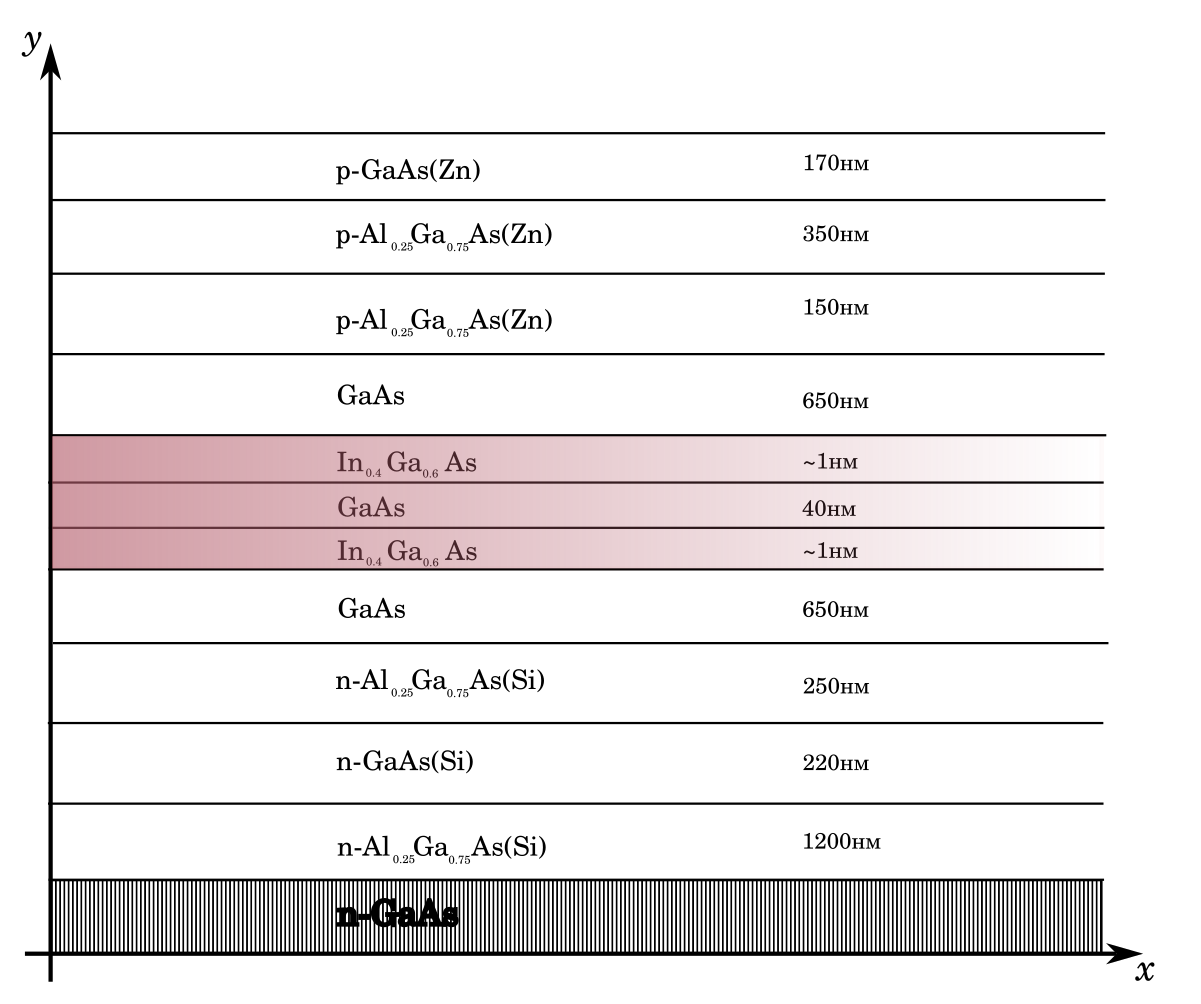
\includegraphics[width=0.5\textwidth]{1.png}
		\caption{Cхема системы}
	\end{figure}
	
	\quad При пропускании тока через систему в ней происходят следующей процессы:
	
	\begin{enumerate}
		\item Протекающий в системе ток создаёт в каждом из слоёв источники тепла, мощность которых определяется по закону Джоуля-Ленца. 
		
		\begin{center}
			$q_i = \dfrac{P_i}{S_i} = \dfrac{U_i I}{wd_i}$
		\end{center}
		
		\item Верхний контакт на p-области обменивается теплом с воздухом комнатной температуры. Это условие учитывается в системе в виде:
		
		
		\begin{center}
			$\left( k_9\dfrac{\partial T_9}{\partial y} - \alpha T_9\right)\bigg|_{y=h} = -\alpha T_{air}$
		\end{center}
		
		\item Протекающиий в системе ток создаёт инверсию населённости зарядов в активной области  из-за чего заряды начинают рекомбинировать. Энергия от рекомбинации частично идёт на нагрев, а частично на излучение.  
		
		\begin{center}
			$UI = P_{\text{опт}} + P_{\text{тепл}}$
		\end{center}
		
	\end{enumerate}
	
	\quad Энергия, ушедшая в активной области на излучение, не вся покидает систему. Она может перепоглотиться в других слоях и остаться в системе в виде тепла. Такой эффект характерен для работы лазера в допороговом режиме, при работе же при силе тока выше порога перепоглощение почти не наблюдается. 
	
	\quad Таким образом температура в системе описывается функцией $T = f(x, y, I)$ которую и предстоит найти. Исходя из изложенной выше конфигурации, модеирование распределения температуры сводится к решению стационарного уравнения теплопроводности:
	
	\begin{equation}
		\dfrac{\partial^2 T_i}{\partial x^2} + \dfrac{\partial^2 T_i}{\partial y^2}  = -\dfrac{q_i}{k_i} 
	\end{equation}
	
	\begin{center}
		где $q_i$ тепловой поток $i$-того слоя, а $k_i$ теплопроводность $i$-того слоя. 
	\end{center}
	
	\quad С условиями непрерывности на границе слоёв:
	
	\begin{equation}
		\begin{cases}
			T_i(x, y)\bigg|_{y=y_i} = T_{i-1}(x, y)\bigg|_{y=y_i} \\
			\dfrac{\partial T_i}{\partial y} \bigg|_{y=y_i} = \dfrac{\partial T_{i-1}}{\partial y}\bigg|_{y=y_i} \\
		\end{cases}
	\end{equation}
	
	\quad И граничными условиями: 
	
	\begin{equation}
		\begin{cases}
			\left( k_9\dfrac{\partial T_9}{\partial y} - \alpha T_9\right)\bigg|_{y=h} = -\alpha T_{air} \\
			T(x, y) \bigg|_{y=0} = 293 \\
			\dfrac{\partial T_i}{\partial x} \bigg|_{x=0,w} = 0
		\end{cases}
	\end{equation}
	
	\quad Так получаем полностью определённую краевую задачу на распределение температуры. 
	
	\quad 	\textbf{ \S 2. Общее решение в слое}
	
	\quad Распишем уравнение теполпроводности для каждого слоя:
	
	\begin{equation}
		\frac{\partial^2 T_i}{\partial x^2} + \dfrac{\partial^2 T_i}{\partial y^2} = -\dfrac{q_i}{k_i}
	\end{equation}

	\quad Слои нумеруются здесь снизу вверх, от подложки, которая имеет номер 0, до слоя $GaAs(Zn)$, к которому присоединён провод.
	
	\quad Теперь найдём общее решение уравнения (1), как решение неоднородного линейного диффернциального уравнения. Для этого найдём решение однородной задачи:
	
	\begin{equation}
		\dfrac{\partial^2 T_i}{\partial x^2} + \dfrac{\partial^2 T_i}{\partial y^2} = 0
	\end{equation}
	
	\quad Метод Фурье: $T(x, y) = X(x) Y(y) \implies $
	
	\begin{center}
		$\implies Y(y) \dfrac{d^2 X}{dx^2} + X(x) \dfrac{d^2 Y}{dy^2} = 0 \implies \dfrac{1}{X} \dfrac{d^2 X}{dx^2} = -\dfrac{1}{Y} \dfrac{d^2 Y}{dy^2} = -\lambda $
	\end{center}
	
	\begin{equation}
		\begin{cases}
			\dfrac{d^2 X}{dx^2} + \lambda X = 0 \\
			\\
			\dfrac{d^2 Y}{dy^2} - \lambda Y= 0 
 		\end{cases}
	\end{equation}
	   
	\quad Общее решение первого уравнения системы определяется как:   
	
	\begin{center}
		$X(x) = C_1 e^{i\sqrt{\lambda} x} + C_2 e^{-i\sqrt{\lambda} x} $
	\end{center} 
	
	\quad Подставляем в Г.У.: 
	
	\begin{center}
		$\dfrac{dX}{dx} = i\sqrt{\lambda}C_1e^{i\sqrt{\lambda} x} - i\sqrt{\lambda} C_2 e^{-i\sqrt{\lambda} x} $
		
		$\begin{cases}
			C_1 - C_2 = 0 \\
			C_1 e^{i\sqrt{\lambda} w} - C_2 e^{-i\sqrt{\lambda} w} = 0
		\end{cases} \Leftrightarrow \left[\begin{array}{cc|c}
		1 & -1 & 0 \\
		e^{i\sqrt{\lambda} w} & -e^{-i\sqrt{\lambda} w} & 0
		\end{array} \right]$
		
		$ e^{i\sqrt{\lambda} x} - e^{i\sqrt{\lambda} x} = 0 \implies \sin{\sqrt{\lambda}w} = 0 $
		
		$\lambda_n = \dfrac{\pi^2 n^2}{w^2}, \quad \forall n \in \mathbb{N}\cup\left\{ 0 \right\} $ 
		
		Собственные функции: $X_n (x) = \cos{\dfrac{\pi n x}{w}}$ 
	\end{center}
	
	\quad Теперь мы можем записать общее решение однородной задачи:
	
	\begin{equation}
		T_n (x, y) = Y_n (y) \cos{\dfrac{\pi n x}{w}},\quad \forall n \in \mathbb{N}\cup\left\{ 0 \right\} 
 	\end{equation}
	  
	\begin{equation}
		T(x, y) = \displaystyle\sum\limits_{n=0}^{\infty} Y_n (y) \cos{\dfrac{\pi n x}{w}}
	\end{equation}
	  
	\quad Подставим решение (8) в уравнение (1) и найдём общее решение неоднородной задачи: 
	
	\begin{center}
		$ \dfrac{\partial^2 }{\partial x^2} \left( \displaystyle\sum\limits_{n=0}^{\infty} Y_n (y) \cos{\dfrac{\pi n x}{w}} \right) + \dfrac{\partial^2}{\partial y^2} \left(\displaystyle\sum\limits_{n=0}^{\infty} Y_n (y) \cos{\dfrac{\pi n x}{w}}\right)= -\dfrac{q_i}{k_i}$
		
		$\displaystyle\sum\limits_{n=1}^{\infty} \left( \dfrac{d^2 Y_n}{dy^2} - \lambda_n Y_n \right) \cos{\dfrac{\pi n x}{w} }= -\dfrac{q_i}{k_i}$ 
	\end{center}	
	
	\quad Разложим $g(x) = \dfrac{q_i}{k_i}$ в ряд Фурье по косинусам: $\dfrac{q_i}{k_i} = \displaystyle\sum\limits_{n=0}^{\infty} C_n \cos{\dfrac{\pi n x}{w}}$
	
	\begin{center}
		$C_n = \dfrac{\left<\dfrac{q_i}{k_i} \bigg| \cos{\dfrac{\pi n x}{w}}\right>}{\| \cos{\dfrac{\pi n x}{w}}\|^2}$, $\| \cos{\dfrac{\pi n x}{w}}\|^2 = \dfrac{w}{2}$
		
		$\left<\dfrac{q_i}{k_i}\bigg|\cos{\dfrac{\pi n x}{w}}\right> = \displaystyle\int\limits_{0}^{w} \dfrac{q_i}{k_i} \cos{\dfrac{\pi n x}{w}} dx = \dfrac{wq_i}{\pi n k_i} \sin{\dfrac{\pi n x}{w}} \bigg|_{0}^{w} = 0$
	\end{center}
	
	\quad В итоге все коэфиценты кроме $C_0 = \dfrac{q_i}{k_i}$ равны нулю, учитывая это: 
	 
	\begin{equation}
		\begin{cases}
			\dfrac{d^2 Y_0}{dy^2} = -\dfrac{q_i}{k_i} \\
			\\
			\dfrac{d^2 Y_n}{dY^2} -\lambda_n Y_n = 0
		\end{cases} \implies Y_n (y) = \begin{cases}
			-\dfrac{q_i }{2k_i} y^2 + C_1 y + C_2 , \quad n = 0 \\
			\\
			A_n \sinh{\dfrac{\pi n y}{w}}+ B_n \cosh{\dfrac{\pi n y}{w}},  \quad \forall n \in \mathbb{N}
		\end{cases}
	\end{equation}
	  
	  
	\quad Таким образом общее решение неоднородной задачи (1) имеет вид: 
	
	\begin{equation}
		T_i(x, y)  = -\dfrac{q_i }{2k_i} y^2 + C^{(i)}_1 y + C^{(i)}_2 + \displaystyle\sum\limits_{n=1}^{\infty} \left(A^{(i)}_n \sinh{\dfrac{\pi n y}{w}}+ B^{(i)}_n \cosh{\dfrac{\pi n y}{w}} \right) \cos{\dfrac{\pi n x}{w}}
	\end{equation}
	
	\quad \textbf{\S3. Поиск частного решения. Задача о нахождении коэфицентов.}
	
	\quad Прежде чем явно искать коэфиценты в формуле (10), подставляя решение в Г. У., заметим следующее: 
	
	\begin{center}
		$T_i (x, y) = T_{i,\text{частн.}} + T_{i,\text{общ}}$
		
		где: $T_{i,\text{частн.}} = -\dfrac{q_i}{2k_i} y^2 + C^{(i)}_1 y + C^{(i)}_2$
		
		$T_{i,\text{общ}} = \displaystyle\sum\limits_{n=1}^{\infty} \left(A^{(i)}_n \sinh{\dfrac{\pi n y}{w}}+ B^{(i)}_n \cosh{\dfrac{\pi n y}{w}} \right) \cos{\dfrac{\pi n x}{w}}$
	\end{center}
	
	\quad Проверим, что $T_{i,\text{частн.}}$ является решением уравнения (1): 
	
	\begin{center}
		$\dfrac{\partial^2 T}{\partial x^2 } + \dfrac{\partial^2 T}{\partial y^2} = \dfrac{\partial^2 }{\partial y^2 } \left( -\dfrac{q_i}{2k_i} y^2 + C^{i}_1 y + C^{i}_2\right) = -\dfrac{q_i}{k_i} \equiv -\dfrac{q_i}{k_i}$
	\end{center}
	
	\quad Точно также и $T_{i,\text{общ}}$ является решеим уравнения (5). Это значит, что задачу о нахождении коэфицентов можно разбить на две задачи для двух решений, предполагая, что у решений те же свойства непрерывности, что и у общего решения (10). Отдельное внимание тут стоит уделить лишь условиям на границе структуры (3). Рассмотрим сначала нижнее:
	
	\begin{equation}
		T_{i} \bigg|_{y=0} = T_{i,\text{частн.}} \bigg|_{y=0} + T_{i, \text{общ.}}\bigg|_{y=0} = 293
	\end{equation}
	
	\quad Условие (11) необходимо разбить на два уравнения из следующей идеи. Пусть неоднородное решение будет полностью согласовано с температурой на дне структуры, а для общего однородного решения поставим новое искусственное однородное условие $T_{i, \text{общ.}} = 0$. Тогда условие (11) разобьётся на два уравнения:
	
	\begin{equation}
		\begin{cases}
			T_{i,\text{частн.}} \bigg|_{y=0} = 293 \\
			T_{i, \text{общ.}}\bigg|_{y=0} = 0\\
		\end{cases}
	\end{equation}
	
	\quad Похожим образом поступим с условием на p-контакте. 
	
	\begin{center}
		$\begin{cases}
			\left(k_9 \dfrac{\partial T_{9, \text{частн}}}{\partial y} - \alpha T_9\right)\bigg|_{y=h} = -293\alpha \\
			T_i (x, y)\bigg|_{y_i} = T_{i-1} (x, y)\bigg|_{y_i} \\
			k_i \dfrac{\partial T_i}{\partial y} \bigg|_{y_i} = k_{i-1} \dfrac{\partial T_{i-1}}{\partial y}\bigg|_{y_i} \\
			T_{0, \text{частн}}\bigg|_{y=0} = 0
		\end{cases}$
	\end{center}
	
\end{document}